\begin{enumerate}[label=\arabic*.,ref=\theenumi]
\numberwithin{equation}{enumi}
\item The op amp in the circuit of Fig. \ref{fig:ee18btech11028_2_q} has an open-loop gain of $10^{5}$ and a single-pole rolloff with $\omega_{3dB}$ = 10 rad/s.

%\renewcommand{\thefigure}{\theenumi.\arabic{figure}}
%
\begin{figure}[!ht]
	\begin{center}
		\resizebox{\columnwidth}{!}{\begin{circuitikz}
\ctikzset{bipoles/length=1cm}

\draw 
(0, 0) node[op amp] (opamp) {}
(opamp.-) -- (-2.5,0.35) to[R,l_=$R_1$,*-*] (-3.5, 0.35) to (-4, 0.35) to (-4.5, 0.35) node[ground]{}
(opamp.-) --(-0.9,1) to[R=$R_2$] (1,1) -- (1,0) --(2,0) node at(2.3,0){$V_0$}
(opamp.out) to (1.5,0)--(1.5,-0.5) to[R=$R_L$] (1.5,-1.5) to (1.5,-1.5) node[ground]{}
(opamp.+) -- (-0.6,-0.35) to[R =$R_s$,*-*] (-2.6,-0.35) to[V=$V_s$] (-2.6,-2.4) node[ground]{}
node at(-3.5,0.1){$-$}
node at(-2.5,0.1){$+$}
node at(-3,-0.1){$V_f$}
;\end{circuitikz}

}
	\end{center}
\caption{}
\label{fig:ee18btech11028_2_q}
\end{figure}
%
\begin{table}[!ht]
    \centering
    

%%  This section checks if we are begin input into another file or  %%
%%  the file will be compiled alone. First use a macro taken from   %%
%%  the TeXbook ex 7.7 (suggestion of Han-Wen Nienhuys).            %%
\def\ifundefined#1{\expandafter\ifx\csname#1\endcsname\relax}


%%  Check for the \def token for inputed files. If it is not        %%
%%  defined, the file will be processed as a standalone and the     %%
%%  preamble will be used.                                          %%
\ifundefined{inputGnumericTable}

%%  We must be able to close or not the document at the end.        %%
	\def\gnumericTableEnd{\end{document}}


%%%%%%%%%%%%%%%%%%%%%%%%%%%%%%%%%%%%%%%%%%%%%%%%%%%%%%%%%%%%%%%%%%%%%%
%%                                                                  %%
%%  This is the PREAMBLE. Change these values to get the right      %%
%%  paper size and other niceties.                                  %%
%%                                                                  %%
%%%%%%%%%%%%%%%%%%%%%%%%%%%%%%%%%%%%%%%%%%%%%%%%%%%%%%%%%%%%%%%%%%%%%%

	\documentclass[12pt%
			  %,landscape%
                    ]{report}
       \usepackage[latin1]{inputenc}
       \usepackage{fullpage}
       \usepackage{color}
       \usepackage{array}
       \usepackage{longtable}
       \usepackage{calc}
       \usepackage{multirow}
       \usepackage{hhline}
       \usepackage{ifthen}
%%  End of the preamble for the standalone. The next section is for %%
%%  documents which are included into other LaTeX2e files.          %%
\else

%%  We are not a stand alone document. For a regular table, we will %%
%%  have no preamble and only define the closing to mean nothing.   %%
    \def\gnumericTableEnd{}

%%  If we want landscape mode in an embedded document, comment out  %%
%%  the line above and uncomment the two below. The table will      %%
%%  begin on a new page and run in landscape mode.                  %%
%       \def\gnumericTableEnd{\end{landscape}}
%       \begin{landscape}


%%  End of the else clause for this file being \input.              %%
\fi

%%%%%%%%%%%%%%%%%%%%%%%%%%%%%%%%%%%%%%%%%%%%%%%%%%%%%%%%%%%%%%%%%%%%%%
%%                                                                  %%
%%  The rest is the gnumeric table, except for the closing          %%
%%  statement. Changes below will alter the table's appearance.     %%
%%                                                                  %%
%%%%%%%%%%%%%%%%%%%%%%%%%%%%%%%%%%%%%%%%%%%%%%%%%%%%%%%%%%%%%%%%%%%%%%

\providecommand{\gnumericmathit}[1]{#1} 
%%  Uncomment the next line if you would like your numbers to be in %%
%%  italics if they are italizised in the gnumeric table.           %%
%\renewcommand{\gnumericmathit}[1]{\mathit{#1}}
\providecommand{\gnumericPB}[1]%
{\let\gnumericTemp=\\#1\let\\=\gnumericTemp\hspace{0pt}}
 \ifundefined{gnumericTableWidthDefined}
        \newlength{\gnumericTableWidth}
        \newlength{\gnumericTableWidthComplete}
        \newlength{\gnumericMultiRowLength}
        \global\def\gnumericTableWidthDefined{}
 \fi
%% The following setting protects this code from babel shorthands.  %%
 \ifthenelse{\isundefined{\languageshorthands}}{}{\languageshorthands{english}}
%%  The default table format retains the relative column widths of  %%
%%  gnumeric. They can easily be changed to c, r or l. In that case %%
%%  you may want to comment out the next line and uncomment the one %%
%%  thereafter                                                      %%
\providecommand\gnumbox{\makebox[0pt]}
%%\providecommand\gnumbox[1][]{\makebox}

%% to adjust positions in multirow situations                       %%
\setlength{\bigstrutjot}{\jot}
\setlength{\extrarowheight}{\doublerulesep}

%%  The \setlongtables command keeps column widths the same across  %%
%%  pages. Simply comment out next line for varying column widths.  %%
\setlongtables

\setlength\gnumericTableWidth{%
	60pt+%
	100pt+%
0pt}
\def\gumericNumCols{2}
\setlength\gnumericTableWidthComplete{\gnumericTableWidth+%
         \tabcolsep*\gumericNumCols*2+\arrayrulewidth*\gumericNumCols}
\ifthenelse{\lengthtest{\gnumericTableWidthComplete > \linewidth}}%
         {\def\gnumericScale{\ratio{\linewidth-%
                        \tabcolsep*\gumericNumCols*2-%
                        \arrayrulewidth*\gumericNumCols}%
{\gnumericTableWidth}}}%
{\def\gnumericScale{1}}

%%%%%%%%%%%%%%%%%%%%%%%%%%%%%%%%%%%%%%%%%%%%%%%%%%%%%%%%%%%%%%%%%%%%%%
%%                                                                  %%
%% The following are the widths of the various columns. We are      %%
%% defining them here because then they are easier to change.       %%
%% Depending on the cell formats we may use them more than once.    %%
%%                                                                  %%
%%%%%%%%%%%%%%%%%%%%%%%%%%%%%%%%%%%%%%%%%%%%%%%%%%%%%%%%%%%%%%%%%%%%%%

\ifthenelse{\isundefined{\gnumericColA}}{\newlength{\gnumericColA}}{}\settowidth{\gnumericColA}{\begin{tabular}{@{}p{60pt*\gnumericScale}@{}}x\end{tabular}}
\ifthenelse{\isundefined{\gnumericColB}}{\newlength{\gnumericColB}}{}\settowidth{\gnumericColB}{\begin{tabular}{@{}p{100pt*\gnumericScale}@{}}x\end{tabular}}
\begin{tabular}[c]{%
	b{\gnumericColA}%
	b{\gnumericColB}%%
	}

%%%%%%%%%%%%%%%%%%%%%%%%%%%%%%%%%%%%%%%%%%%%%%%%%%%%%%%%%%%%%%%%%%%%%%
%%  The longtable options. (Caption, headers... see Goosens, p.124) %%
%	\caption{The Table Caption.}             \\	%
% \hline	% Across the top of the table.
%%  The rest of these options are table rows which are placed on    %%
%%  the first, last or every page. Use \multicolumn if you want.    %%

%%  Header for the first page.                                      %%
%	\multicolumn{3}{c}{The First Header} \\ \hline 
%	\multicolumn{1}{c}{colTag}	%Column 1
%	&\multicolumn{1}{c}{colTag}	%Column 2
%	&\multicolumn{1}{c}{colTag}	\\ \hline %Last column
%	\endfirsthead

%%  The running header definition.                                  %%
%	\hline
%	\multicolumn{3}{l}{\ldots\small\slshape continued} \\ \hline
%	\multicolumn{1}{c}{colTag}	%Column 1
%	&\multicolumn{1}{c}{colTag}	%Column 2
%	&\multicolumn{1}{c}{colTag}	\\ \hline %Last column
%	\endhead

%%  The running footer definition.                                  %%
%	\hline
%	\multicolumn{3}{r}{\small\slshape continued\ldots} \\
%	\endfoot

%%  The ending footer definition.                                   %%
%	\multicolumn{3}{c}{That's all folks} \\ \hline 
%	\endlastfoot
%%%%%%%%%%%%%%%%%%%%%%%%%%%%%%%%%%%%%%%%%%%%%%%%%%%%%%%%%%%%%%%%%%%%%%

\hhline{|-|-}
	 \multicolumn{1}{|p{\gnumericColA}|}%
	{\gnumericPB{\centering}\textbf{Parameters}}
	&\multicolumn{1}{p{\gnumericColB}|}%
	{\gnumericPB{\centering}\textbf{Value}}

	
\\


\hhline{|--|}
	 \multicolumn{1}{|p{\gnumericColA}|}%
	{\gnumericPB{\centering}$P_{1}$}
	&\multicolumn{1}{p{\gnumericColB}|}%
	{\gnumericPB{\centering}$2\pi  10^{6}$ rad/sec}


\\


\hhline{|--|}
	 \multicolumn{1}{|p{\gnumericColA}|}%
	{\gnumericPB{\centering}$P_{2}$}
	&\multicolumn{1}{p{\gnumericColB}|}%
	{\gnumericPB{\centering}$2\pi  10^{7}$ rad/sec}


\\

\hhline{|--|}
	 \multicolumn{1}{|p{\gnumericColA}|}%
	{\gnumericPB{\centering}$P_{3}$}
	&\multicolumn{1}{p{\gnumericColB}|}%
	{\gnumericPB{\centering}$2\pi  10^{8}$ rad/sec}


\\



\hhline{|--|}
	 \multicolumn{1}{|p{\gnumericColA}|}%
	{\gnumericPB{\centering}$G_0$}
	&\multicolumn{1}{p{\gnumericColB}|}%
	{\gnumericPB{\centering}$10^{4}$}



\\
\hhline{|-|-|}
\end{tabular}

\ifthenelse{\isundefined{\languageshorthands}}{}{\languageshorthands{\languagename}}
\gnumericTableEnd

    \caption{}
    \label{table:ee18btech11028_2_parameters}
\end{table}

\item Sketch a Bode plot for the loop gain.
\\
\solution
Op-amp in our question has an open loop gain characterised by a single pole $P_{11} $ from table \ref{table:ee18btech11028_2_parameters} i.e.
\begin{align}
    G(s) = \frac{10^5}{1 + \frac{s}{P_{11}}}
        \label{eq:ee18btech11028_2_2}
\end{align}

Using voltage division on Fig. \ref{fig:ee18btech11028_2_q} we obtain,
\begin{align}
    H(s) = \frac{V_{f}}{V_{o}}
     &= \frac{\frac{1}{sC_{f}}}{R_{f} + \frac{1}{sC_{f}}}
    \\
    \implies H(s) = \frac{1}{1 + \frac{s}{P_{21}}}
        \label{eq:ee18btech11028_2_1}
\end{align}
where, 
\begin{align}
    P_{21} = \frac{1}{R_{f}C_{f}} = 1000
\end{align}

The loop gain, 
\begin{align}
    GH(s) = \frac{10^5}{(1+\frac{s}{10})(1 + \frac{s}{1000})}
\end{align}

\begin{figure}[!ht]
    \centering
    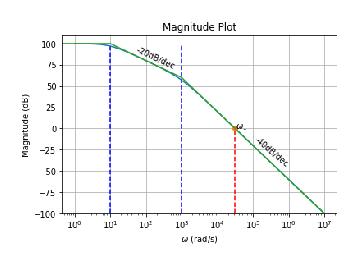
\includegraphics[width=\columnwidth]{./figs/ee18btech11028/ee18btech11028_2_1.eps}
    \caption{Magnitude plot}
    \label{fig:ee18btech11026_2_1}
\end{figure}


\begin{figure}[!ht]
    \centering
    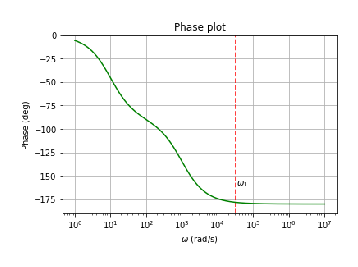
\includegraphics[width=\columnwidth]{./figs/ee18btech11028/ee18btech11028_2_2.eps}
    \caption{Phase plot}
    \label{fig:ee18btech11026_2_2}
\end{figure}


\item Find the frequency at which $ |GH|= 1$, and find the corresponding phase margin.
\\
\solution
Value of $\omega$ for unity magnitude can be obtained from Fig. \ref{fig:ee18btech11026_2_1} which is approximately $3 \times 10^{4}$.
More precise value can be obtained by solving for $\omega$ in,
\begin{align}
    \frac{10^{5}}{\sqrt{1 + \frac{w_{1}^{2}}{P_{1}^{2}}} \sqrt{1 + \frac{w_{1}^{2}}{P_{2}^{2}}}} = 1
\end{align}

Thus, 

\begin{align}
     \omega_{1} = 3.15 \times 10^{4} rad/s
\end{align}
The phase margin visibly from the Fig. \ref{fig:ee18btech11026_2_2} is very small.
\begin{align}
    PM = 180 \degree - \tan^{-1}(\frac{\omega_{1}}{10}) - \tan^{-1}(\frac{\omega_{1}}{1000})
      & = 1.84 \degree
\end{align}

\item Find the closed-loop transfer function, including its zero
and poles. Sketch a pole-zero plot. Sketch the magnitude of
the transfer function versus frequency, and label the important parameters on your sketch.
\\ 
\solution

\begin{align}
    T(s) = \frac{G(s)}{1 + G(s)H(s)}
    \\
\end{align}

From \eqref{eq:ee18btech11028_2_1} and \eqref{eq:ee18btech11028_2_2} we have,
\begin{align}
    \implies T(s) = \frac{10^{6}(s+1000)}{s^{2} + 1010s + 10^{4} + 10^{9}}
    \\
\end{align}

Zeros of closed loop transfer function,
\begin{align}
    Z_{1} = -1000
\end{align}

Similarly for poles,
\begin{align}
    s^{2} + 1010s + 10^{4} + 10^{9} = 0
    \\
    \implies P_{1}, P_{2} = -505 \pm j31618.9
\end{align}

\begin{figure}[!ht]
    \centering
    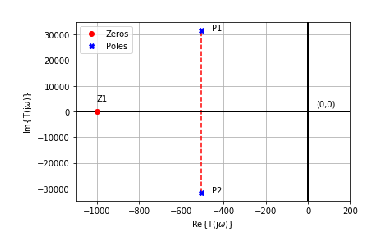
\includegraphics[width=\columnwidth]{./figs/ee18btech11028/ee18btech11028_2_3.eps}
    \caption{Pole zero plot}
    \label{fig:ee18btech11026_2_3}
\end{figure}


\begin{figure}[!ht]
    \centering
    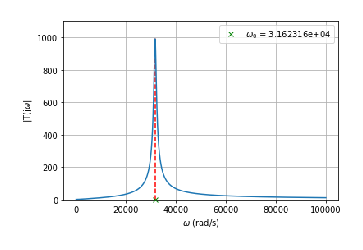
\includegraphics[width=\columnwidth]{./figs/ee18btech11028/ee18btech11028_2_4.eps}
    \caption{Closed loop magnitude plot}
    \label{fig:ee18btech11026_2_4}
\end{figure}

Poles are at $\omega_{0} = 3.16 \times 10^{4}$


\end{enumerate}